\documentclass[10pt]{beamer}
\usepackage[utf8]{inputenc}
\usepackage[dvipsnames]{xcolor}
\usepackage{charter}
\usepackage{amsmath}
\usepackage{amsfonts}
\usepackage{mathtools}
\usepackage{amssymb}
\usepackage{hyperref}
\usepackage[ruled,vlined]{algorithm2e}
\usepackage{commath}

\title{Variance reduced methods in Deep Neural Networks}
\author{Alexander Apostolov}
\institute {École Polytechnique Fédérale de Lausanne}
\date{November 11th 2020}

\begin{document}


\frame{\titlepage}


\begin{frame}{Goal of this semester project}

Analyze the effect of \alert{variance reduction methods} in \alert{deep neural networks}.
\newline
\begin{itemize}
    \item Analysis of SGD, Adam, AdaGrad, SVRG and STORM on a small NN.
    \item Analysis and trying to get insights about possibilities of using better performance of variance reduction methods on deep neural networks. 
\end{itemize}
    
\end{frame}

\begin{frame}
\frametitle{Why variance reduction methods?}
\begin{itemize}
    \item In machine learning, the following optimization is often encountered:\
    Let $f_1, f_2, \dots, f_n$ be a sequence of vector functions from $\mathbb{R}^d$ to $\mathbb{R}$.
    The goal is to find a solution to the following optimization problem:
    $$\min F(w),~~F(w)=\frac{1}{n}\sum_{i=1}^n f_i(w)$$
    \item \textbf{Gradient Descent (GD)} is a standard method to solve this:
    $$w^{(t)} = w^{(t-1)} - \eta_t \nabla F(w^{(t-1)})$$
    \item Each iteration requires computation of the whole gradient, this is why \textbf{Stochastic Gradient Descent (SGD)} which decrease computational cost by $\frac{1}{n}$ per iteration has been widely adopted:
    $$w^{(t)} = w^{(t)} -\eta_t \nabla f_{i_t}(w^{(t-1)})$$
\end{itemize}
\end{frame}

\begin{frame}{Why variance reduction methods?}
    Randomness in SGD introduces variance which slows down convergence. This creates a trade off between fast per iteration computation and fast convergence.
    
    \vspace{5mm}
    \textbf{Variance reduced methods} allows keeping fast convergence at fast per iteration speed. We will analyze two methods:
    \begin{itemize}
        \item \textbf{Stochastic Variance Reduced Gradient (SVRG)}
        \item \textbf{STOchastic Recursive Mometum STORM}
    \end{itemize}
    
\end{frame}

\begin{frame}{SVRG}
    Each iteration of SVRG is given by:
    $$w^{(t)} = w^{(t)} -\eta_t(\nabla f_{i_t}(w^{(t-1)}) - \nabla f_{i_t}(\Tilde{w}) + \Tilde{\mu})$$
    where $\Tilde{w}$ is snapshot of $w$ we make every $m$ iterations and :
    $$\Tilde{\mu} = \nabla F(\Tilde{w}) = \frac{1}{n}\sum_{i=1}^n \nabla f_i(\Tilde{w})$$
    
    Notice that: 
    \begin{itemize}
        \item $\nabla f_{i_t}(w^{(t-1)}) - \nabla f_{i_t}(\Tilde{w}) + \Tilde{\mu}$ is an unbiased estimate of $\nabla P(w)$:
    $$\mathbb{E}[w^{(t)} | w^{(t-1)}] = w^{(t-1)}-\eta_t \nabla F(w^{(t-1)})$$
        \item Variance is reduced. When $\Tilde{w}$ and $w^{(t)}$ both converge to $w_{\ast}$, then $\Tilde{\mu} \rightarrow 0$. If $\nabla f_i(\Tilde{w}) \rightarrow \nabla f_i(w_{\ast})$, then:
        $$\nabla f_i(w^{(t-1)}) - \nabla f_i(\Tilde{w}) + \Tilde{\mu} \rightarrow \nabla f_i(w^{(t-1)}) - \nabla f_i(w_{\ast}) \rightarrow 0$$
    \end{itemize}
\end{frame}


\begin{frame}{SVRG}
    \begin{algorithm}[H]
        \DontPrintSemicolon
        \SetAlgoNoLine

        \KwIn{learning rate $\eta$ and update frequency $m$}
        \textbf{Initialize} $\Tilde{w}_0$\;
        \For{$s \leftarrow 1, 2, \dots$}{
          $\Tilde{w} \gets \tilde{w}_{s-1}$\;
          $\Tilde{\mu} \gets \frac{1}{n}\sum_{i=1}^n \nabla f_i(\Tilde{w})$\;
          $w_0 \gets \tilde{w}$\;
          \For{$t \leftarrow 1,2\dots, n$}{
            Randomly pick $i_t \in \{1, \dots, n\}$  
            
            $w^{(t)} \gets w^{(t)} -\eta(\nabla f_{i_t}(w^{(t-1)}) - \nabla f_{i_t}(\Tilde{w}) + \Tilde{\mu})$
          }
          \textbf{Save snapshot} $\tilde{w}_s \gets w_m$\;
        }
        \caption{{\textsc{SVRG Procedure}}}
        \label{algo:svrg}
    \end{algorithm}
\end{frame}

\begin{frame}{STORM}
    Each iteration of STORM is given by:
    $$d^{(t)} = (1-a)d^{(t-1)} + a\nabla f_{i_t}(w^{(t)}) + (1-a)(\nabla f_{i_t}(w^{(t)}) +  \nabla f_{i_t}(w^{(t-1)}))$$
    $$w^{(t+1)} = w^{(t)} - \eta d_t$$
    Notice that:
    \begin{itemize}
        \item When $w^{(t)} \approx w^{(t-1)}$, then the last term of the first equality tends to 0. Then the update is exactly the same as SGD with momentum. 
    \end{itemize}
\end{frame}

\begin{frame}{STORM}
    \begin{algorithm}[H]
        \DontPrintSemicolon
        \SetAlgoNoLine

        \KwIn{Hyperparameters $k, w, c$}
        \textbf{Initialize} $w_1$\;
        $G_1 \gets \norm {\nabla f_{i_1}(w_1)}$\;
        $d_1 \gets \nabla f_{i_1}(w_1)$\;
        \For{$t \leftarrow 1, 2, \dots$}{
          $\eta_t  \gets \frac{k}{(w+\sum_{i=1}^tG_t^2)^{1/3}}$\;
          $w_{t+1} \gets w_t - \eta_t d_t$\;
          $a_{t+1} \gets c\eta_t^2$\;
          $G_{t+1} \gets \norm{\nabla f_{i_{t+1}}(w_{t+1})}$\;
          $d_{t+1} \gets \nabla f_{i_{t+1}}(w_{t+1}) + (1-a_{t+1})(d_t - \nabla f_{i_{t+1}}(w_t))$\;
        }
        \caption{{\textsc{STORM Procedure}}}
        \label{algo:storm}
    \end{algorithm}
\end{frame}


\begin{frame}{SVRG vs STORM}
\begin{itemize}
    \item Both algorithms need two gradient computations per iteration.
    \item SVRG needs a full gradient computation every m steps (every 5 epochs in non-convex problems).
    \item difficult to get insight on hyperparameters $k,w \text{ and } c$ in STORM.
    \item More hyperparameters to tune for STORM.
\end{itemize}
\end{frame}

\begin{frame}{Baseline comparison}
    We first performed a baseline comparison on MNIST on LeNet for the following algorithms:
    \begin{itemize}
        \item Adam
        \item SGD
        \item AdaGrad
        \item SVRG
        \item STORM
    \end{itemize}
\end{frame}

\begin{frame}{Setup CV}
    \begin{figure}
        \centering
    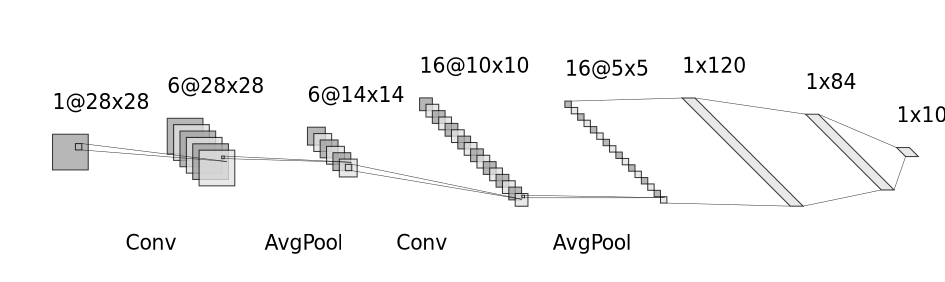
\includegraphics[scale=0.4]{midterm presentation/images/LeNet.png}
        \label{fig:lenet}
        \caption{LeNet network used for MNIST}
    \end{figure} 
\end{frame}

\begin{frame}{Cross-validation for Hyperparameter selection}
    We performed 4-Fold cross-validation on MNIST with LeNet:
    \begin{itemize}
        \item \textbf{Adam} : gridsearch for $\eta \in \{10^{-5}, 10^{-4}, 10^{-3}, 0.01, 0.1\}$ \newline
        Best value : $\eta = 10^{-4}$
        \item \textbf{SGD} : gridsearch for $\eta \in \{10^{-5}, 10^{-4}, 10^{-3}, 0.01, 0.1\}$ \newline
        Best value : $\eta = 0.1$
        \item \textbf{AdaGrad} : gridsearch for $\eta \in \{10^{-4}, 10^{-3}, 0.01, 0.1\}$ \newline
        Best value : $\eta = 0.1$
        \item \textbf{SVRG} : gridsearch for $\eta \in \{10^{-5}, 10^{-4}, 10^{-3}, 0.01, 0.1\}$ \newline
        Best value : $\eta = 0.01$
        \item \textbf{STORM} : gridsearch for $c \in \{10^{-5}, 10^{-4}, 10^{-3}, 0.01, 0.1\}$ and $k \in \{10^{-3}, 0.01, 0.1, 1\}$\newline
        Best value : $c = 100$ and $k=0.1$
        
    \end{itemize}
\end{frame}

\begin{frame}{Cross-validation example : Adam}
    \begin{figure}
        \centering
    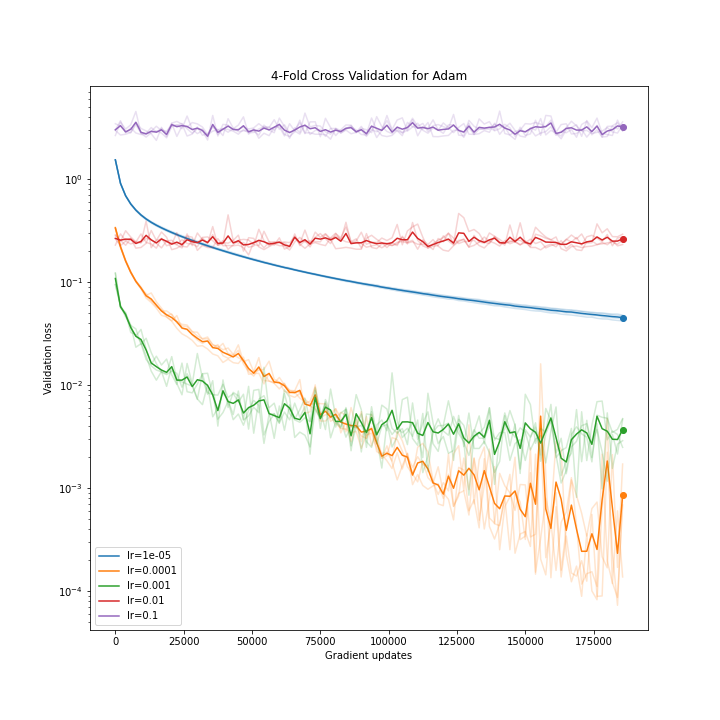
\includegraphics[scale=0.35]{midterm presentation/images/adamCV.png}
        \label{fig:adamCV}
    \end{figure}   
\end{frame}

\begin{frame}{Results on small Neural Network (LeNet)}
    \begin{figure}
        \centering
    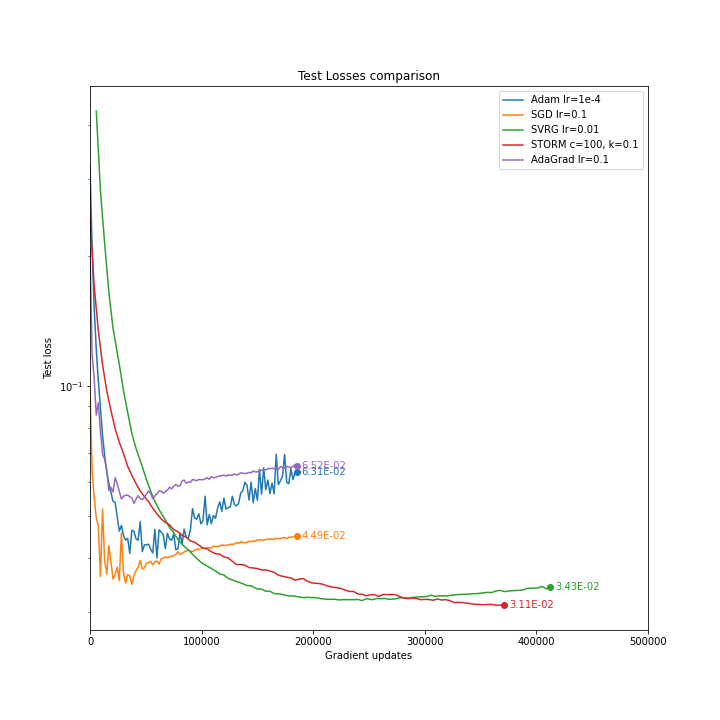
\includegraphics[scale=0.35]{midterm presentation/images/testLossesMnist.png}
        \label{fig:testLossesMnist}
    \end{figure}   
\end{frame}

\begin{frame}{Results on small Neural Network (LeNet)}

    We see that in this setup, \textbf{both variance reduced methods are performing better}.
    \newline
    It takes more time for SVRG and STORM to have better results. This is due in part to the two gradients that have to be computed per iteration and $\tilde{\mu}$ (the full gradient) that has to be computed every 5 iterations in SVRG.

\end{frame}

\begin{frame}{Variance reduced methods on deep neural networks}
    We want to test if variance reduced methods are still performing better on deep neural networks.
    \newline
    The paper "On the Ineffectiveness of Variance Reduced
    Optimization for Deep Learning" by A. Defazio \& L. Bottou suggests that this is not the case, but:
    \begin{itemize}
        \item They just give empirical evidence for specific setups, \textbf{no proofs} that it actually doesn't work.
        \item They \textbf{use Batch-Norm Layers} in their setup. Batch-Norm layers break the assumption that the updates in SVRG are unbiased in expectation.
    \end{itemize}
\end{frame}

\begin{frame}{Our hypothesis}
    We want to check whether \textbf{removing Batch-Norm layers} and using other methods such as MetaInit can \textbf{help SVRG outperform} other algorithms as in the case of the setup with LeNet.
\end{frame}


\begin{frame}{Preliminary algorithm comparison on CIFAR10 with ResNet18}
    To test this hypothesis, we first use ResNet18 on the CIFAR10 dataset to see that in this setup (with BatchNorm layers) SVRG is outperformed.
    \begin{figure}
        \centering
    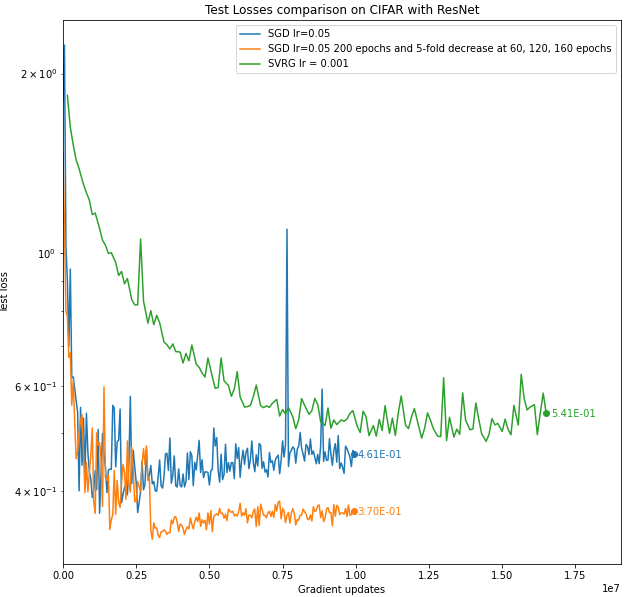
\includegraphics[scale=0.32]{midterm presentation/images/resnet18cifar.png}
        \label{fig:testLossesCifar}
    \end{figure}   
\end{frame}

\begin{frame}{Further steps}
    Plans for the rest of the project:
    \begin{itemize}
        \item Remove BatchNorm layers
        \item Use MetaInit to replace the missing BatchNorm layer
        \item Apply the findings to a deeper network (ResNet50 ?)
    \end{itemize}
\end{frame}

\begin{frame}{ }
\begin{center}
     \Huge Any questions?
\end{center}
   
\end{frame}

\end{document}

